This benchmark is identical to the one presented in Section~\ref{ss:mms_johnbook}
but it is not isoviscous. 
There are three different viscosity fields:
\begin{eqnarray}
\eta_1(x,y) &=& \eta_{min}+(\eta_{max}-\eta_{min})
x^2 (1-x)y^2(1-y)\frac{721}{16} \\
\eta_2(x,y) &=& \eta_{min}+(\eta_{max}-\eta_{min})
\exp [  -10^{13} (x-0.5)^{10} + (y-0.5)^{10}  ] \\
\eta_3(x,y) &=& \eta_{min}+(\eta_{max}-\eta_{min})
\left[1-\exp [  -10^{13} (x-0.5)^{10} + (y-0.5)^{10}  ]\right] 
\end{eqnarray}

\begin{center}
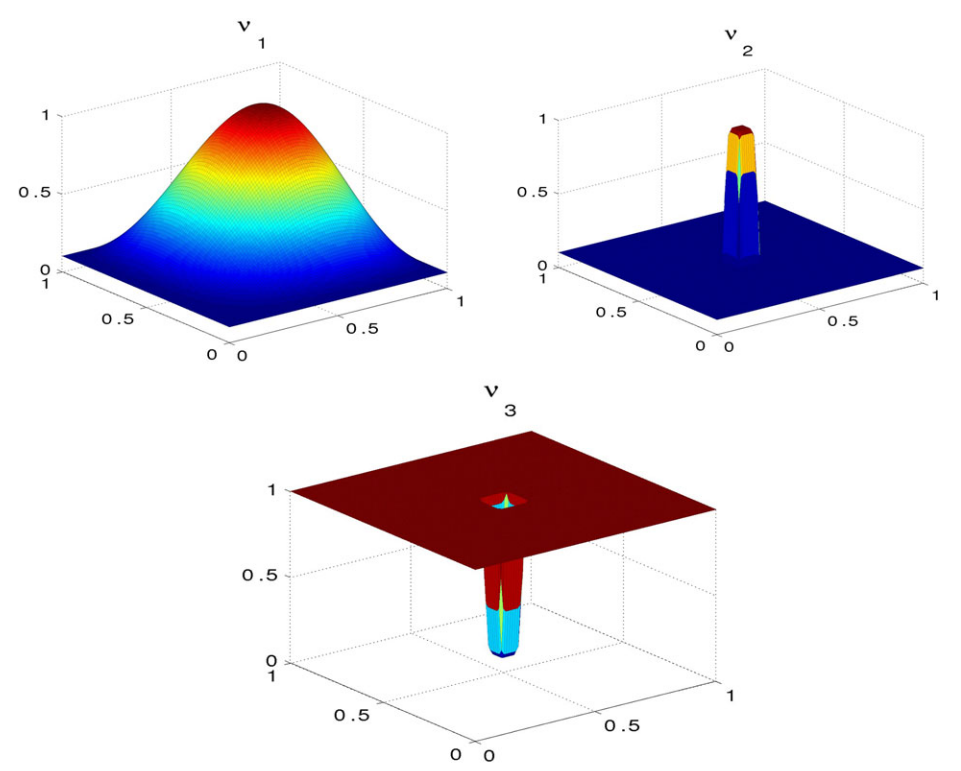
\includegraphics[width=8cm]{images/mms/mms_jokn16b}\\
{\captionfont Taken from \textcite{jokn16b} (2016).}
\end{center}

We have 
\begin{eqnarray}
b_x &=&
\frac{\partial p}{\partial x} 
-2\eta\frac{\partial \dot{\varepsilon}_{xx}}{\partial x}  
-2\eta\frac{\partial \dot{\varepsilon}_{xy}}{\partial y}  
-2 \frac{\partial \eta}{\partial x} \dot{\varepsilon}_{xx}
-2 \frac{\partial \eta}{\partial y} \dot{\varepsilon}_{xy}
\\
b_y &=&
\frac{\partial p}{\partial y} 
-2\eta\frac{\partial \dot{\varepsilon}_{xy}}{\partial x}  
-2\eta\frac{\partial \dot{\varepsilon}_{yy}}{\partial y}  
-2 \frac{\partial \eta}{\partial x} \dot{\varepsilon}_{xy}
-2 \frac{\partial \eta}{\partial y} \dot{\varepsilon}_{yy}
\end{eqnarray}

The three first terms on each line have already been obtained so we 
must focus on the last two:
\begin{eqnarray}
\frac{1}{(\eta_{max}-\eta_{min})}\frac{\partial \eta_1}{\partial x} 
&=& \frac{721}{16} [2x(1-x)-x^2] y^2(1-y)\\
\frac{1}{(\eta_{max}-\eta_{min})}\frac{\partial \eta_1}{\partial y} 
&=& \frac{721}{16} x^2 (1-x)[2y(1-y)-y^2]\\
\frac{1}{(\eta_{max}-\eta_{min})}\frac{\partial \eta_2}{\partial x} 
&=& -10^{14} (x-0.5)^{9} \exp [  -10^{13} (x-0.5)^{10} + (y-0.5)^{10}  ] \\
\frac{1}{(\eta_{max}-\eta_{min})}\frac{\partial \eta_2}{\partial y} 
&=& -10^{14} (y-0.5)^{9} \exp [  -10^{13} (x-0.5)^{10} + (y-0.5)^{10}  ] \\
\frac{1}{(\eta_{max}-\eta_{min})}\frac{\partial \eta_3}{\partial x} 
&=& 10^{14} (x-0.5)^{9} \exp [  -10^{13} (x-0.5)^{10} + (y-0.5)^{10}  ] \\
\frac{1}{(\eta_{max}-\eta_{min})}\frac{\partial \eta_3}{\partial y} 
&=& 10^{14} (y-0.5)^{9} \exp [  -10^{13} (x-0.5)^{10} + (y-0.5)^{10}  ] 
\end{eqnarray}
with 
\begin{eqnarray}
u(x,y) &=&  1000 x^2(1-x)^4  y^2 (3-5y) (1-y) \\
v(x,y) &=& -1000 2x(1-3x) (1-x)^3  y^3(1-y)^2 \\
p(x,y) &=& \pi^2 [xy^3 \cos(2\pi x^2 y) - x^2y \sin(2\pi xy) ]+1/8
\end{eqnarray}

Note that between John's book and the papers \cite{jokn16b} and \cite{jokn18}
there seems to be a small difference: $xy^2$ vs. $xy^3$.
Also the papers have -1/8 while it should be +1/8 (thank you Wolfram Alpha).
